\chapter{Protokol MIDI}\label{chpt:MIDI}

Tento protokol umožňuje přenos zejména hudebních informací mezi dvěma (i~více) elektronickými hudebními nástroji, sekvencery, počítači a~dalšími přístroji. Původně byl zamýšlen pro použití \uv{v~reálném čase}, tedy při živé produkci. \cite{MIDIspecs} S~nástupem moderních \acs{DAW}\footnote{\acl{DAW}} ale přišla možnost povely také nahrávat, upravovat a znovu přehrávat. 

\acs{MIDI} se však netýká výhradně hudby a~hudebních dat. Umožňuje též přenos kontrolních povelů a~synchronizačních značek. Přirozeně se tedy rozšířilo i~do nahrávacích studií, divadel a~dalších zařízení, kde umožňuje globální řízení jednotlivých přehrávačů nebo vzdálené ovládání parametrů řídících konzolí. 

\section{Hardwarová vrstva}
Pro přenos \acs{MIDI} dat se tradičně používá zásuvka a~vidlice \texttt{DIN~5}\footnote{Dnes je častější využití USB sběrnice nebo technologie Bluetooth pro obousměrný přenos.}.  Kabel mezi dvěma zařízeními by neměl být delší než 15\,\unit{m} a~tvořit by jej měla stíněná kroucená dvojlinka. Toto stínění by mělo být připojeno k~\texttt{pinu~2} na obou koncích. 

Výměna informací je realizována pomocí 5\unit{mA} proudové smyčky. Při protékání proudu je zaznamenána \texttt{logická~0}, v~opačném případě \texttt{logická~1}. \cite{MIDIspecs}

Přesná specifika obvodů pro zpracování příchozích a~odchozích \acs{MIDI} signálů upravuje kapitola \emph{Hardware} z~dokumentu \cite{MIDIspecs}. Tato pasáž byla v roce 2014 aktualizována normou \cite{MIDIupd}, která adaptovala protokol i~pro zařízení s~3,3\unit{V} logikou a přidává další prvky pro zamezení zejména \acs{RF}\footnote{\acl{RF}} interferencí. V~následujících schématech bude však zobrazeno originální schéma z~původní normy, 

\subsection{MIDI výstup}

Výstupní port \acs{MIDI} sběrnice je ve své podstatě jednoduchý. Z~\acs{UART}\footnote{\acl{UART}} čipu jsou přes napěťové sledovače nebo tranzistory vedeny logické impulzy na \texttt{pin~5}, zatímco na \texttt{pin~4} je přivedeno stálé napětí. \texttt{Pin~2} je v~tomto případě uzemněn. \cite{MIDIspecs}

Podle aktualizační normy \cite{MIDIupd} je možné přidat za každý rezistor feritové jádro pro zamezení vysokofrekvenčních interferencí. V~případě použití zařízení s~3,3\unit{V} logikou jsou pak použity rezistory s~menšími hodnotami odporů. Na~obr.~\ref{fig:schMIDIout} je schéma k~nahlédnutí.

\begin{figure}[h]
    \centering
    \begin{circuitikz}
    \draw (0,0) circle(0.5cm) ++ (0,-0.9) node {MIDI OUT};
    \draw (0,0.3) circle(0.07cm) node(midi2){} ++(0.1,0.35) node {\tiny 2};
    \draw (-0.3,0) circle(0.07cm) node(midi3){} ++(-0.35,0) node {\tiny 3};
    \draw (0.3,0) circle(0.07cm) node(midi1){} ++(0.35,0) node {\tiny 1};
    \draw (0.22,0.22) circle(0.07cm) node(midi4){} ++(0.32,0.15) node {\tiny 4};
    \draw (-0.22, 0.22) circle(0.07cm) node(midi5){} ++(-0.32,0.15) node {\tiny 5};
    
    \draw (midi2) -- (0,1.5) to[short,-*] (-1,1.5);
    \draw (midi4) -- (0.7,0.7) -- (0.7,2) -- (-2,2);
    \draw (-4,2) node[left]{\small 5\,V} to[short, o-] ++(0,0) to[R=\footnotesize $220\,\Omega$] (-2,2);
    \draw (midi5) -- (-0.7,0.7) -- (-0.7,1) -- (-2,1);
    \draw (-4,1) to[R=\footnotesize $220\,\Omega$] (-2,1);
    
    \draw[densely dashed] (-1.3,1.5) ellipse (0.3 and 0.9);
    \draw (-1.3,0.6) to[short, -*] ++(0,0) node[ground]{};
    
    \draw (-7,1) to[short,o-] (-6.5,1) to[amp] (-5,1) to[amp, t=\small A] (-4,1);
    \draw (-7,1) node[left]{FROM UART};
    
    
\end{circuitikz}
    \caption{Schéma \acs{MIDI} výstupu \cite{MIDIspecs}.}
    \label{fig:schMIDIout}
\end{figure}

\subsection{MIDI vstup}



Vstupní port \acs{MIDI} sběrnice je mnohem složitější. Z~obr.~\ref{fig:schMIDIin} je patrné, že s~cílem eliminovat zemní smyčky, které jsou ve zvukové technice nepřípustné, je vstup každého \acs{MIDI} zařízení skrz optočlen galvanicky oddělen. Z~téhož důvodu je také \texttt{pin~2}~--~na~rozdíl od  výstupního portu~--~zapojen naprázdno (podle~\cite{MIDIspecs}). 

Některá zařízení disponují také výstupem \acs{MIDI} THRU. Ten \uv{kopíruje} data ze vstupu \acs{MIDI} IN a tak umožňuje komplexní řetězení zařízení za sebou. Jeho schéma je totožné s tím na obr. \ref{fig:schMIDIout}.

Aktualizační norma \cite{MIDIupd} pak umožňuje přidání feritových jader za \texttt{piny 4} a \texttt{5}, přes kondenzátor nízké kapacity uzemnění \texttt{pinu 2} a při použití 3,3\unit{V} logiky snížení odporu rezistoru na vstupu optočlenu.

\begin{figure}[h]
    \centering
    \begin{circuitikz}[]
    \draw (0,0) circle(0.5cm) ++ (0,-0.9) node {MIDI IN};
    \draw (0,0.3) circle(0.07cm) node(midi2){} ++(0,0.35) node {\tiny 2};
    \draw (-0.3,0) circle(0.07cm) node(midi3){} ++(-0.35,0) node {\tiny 3};
    \draw (0.3,0) circle(0.07cm) node(midi1){} ++(0.35,0) node {\tiny 1};
    \draw (0.22,0.22) circle(0.07cm) node(midi4){} ++(0.32,0.15) node {\tiny 4};
    \draw (-0.22, 0.22) circle(0.07cm) node(midi5){} ++(-0.32,0.15) node {\tiny 5};
    
    \draw (midi4) -- (0.7,0.7) -- (0.7,1) -- (2,1);
    \draw (midi5) -- (-0.7,0.7) -- (-0.7,2) -- (2,2);
    
    \draw[densely dashed] (1.5,1.5) ellipse (0.3 and 0.9);
    \draw (1.5,0.6) to[short, -*] ++(0,0) node[ground]{};
    
    \draw (2,2) -- (4,2);
    \ctikzset{resistors/scale=0.7}
    \draw (2,1) to[R=\footnotesize $220\,\Omega$] (4,1);
    
    \ctikzset{diodes/scale=0.5}
    \draw (4,2) to [short,-*] ++(0,0) to[D*] (4,1) to[short, -*] ++(0,0) node[below]{\tiny 1N914};
    
    \draw (4,2) -- (5,2);
    \draw (4,1) -- (5,1);
    
    \draw[thick] (5,0.75) rectangle (7,2.25);
    \draw (6,0.75) node[below]{\tiny 6N138};
    
    \draw[densely dashed] (5,2) -- (5.5,2) -- (5.5,1) -- (5,1);
    \draw (5.5,1.5) to[D*] ++(0,0);
    
    \draw[thick, ->] (5.8,1.5) -- (6.3,1.5);
    
    \draw[very thick] (6.5,2) -- (6.5,1);
    \draw (6.5,1.5) -- (6.75,2)  to[short, -*] ++(1.25,0) to[short,-o] ++(1,0) node[right]{TO UART};
    \draw (6.5,1.5) to[short, i=$ $] (6.75,1) -- ++(0.5,0) -- (7.25,0.6) node[ground]{};
    
    \draw (6,2.25) to[short,-o] ++(0,1) node[above]{\small 5\,V};
    \draw (6,2.75) to[short,*-] ++(0,0) to[R=\footnotesize $280\,\Omega$] ++(2,0) to[short, -o] (8,-0.5);
    \draw (8,-0.9) node{MIDI THRU};
    
    %
    %dokument z roku 2014 upravuje:
    %
    
    
    
    
    
\end{circuitikz}
    \caption{Schéma MIDI vstupu \cite{MIDIspecs}.}
    \label{fig:schMIDIin}
\end{figure}

Bude-li do~tohoto vstupu připojen výstup jiného zařízení, které vyšle \linebreak \texttt{logickou~1} objeví se na~\texttt{pinech~4} a~\texttt{5} stejné napětí, v~obvodu tedy neprochází žádný proud~--~\acs{LED}\footnote{\acl{LED}} v~optočlenu nesvítí. Vstupní UART čip přijímá \texttt{logickou~1}. Vyšle-li jiné zařízení \texttt{logickou 0}, na \texttt{pinu~5} poklesne napětí oproti \texttt{pinu~4}, \acs{LED} v optočlenu se rozsvítí, obvodem prochází proud a UART čip přijímá \texttt{logickou~1}.

\section{Softwarová vrstva}\label{chpt:MIDIsw}

\acs{MIDI} protokol přenáší informace (příkazy) po sériové lince přenosovou rychlostí $31 250\,\unit{bps}$. Komunikace je jednosměrná, pro obousměrnou komunikaci je třeba využít dvou rozhraní (vstupu a výstupu) na všech zúčastněných zařízeních. %\cite{MIDIspecs}

Příkazy se skládají z~bajtů, jichž rozeznáváme dva typy:
\begin{itemize}
    \item \texttt{STATUS~BAJT} v~sobě kóduje druh příkazu (\emph{Nota stlačena, Změna kontroléru\ldots}) a~cílový kanál (1-16). 
    \item \texttt{DATA~BAJT} vyjadřuje hodnotu s jakou je příkaz posílán (0-127).
\end{itemize}

\begin{figure}[h]
    \centering
    \begin{subfigure}{.4\textwidth}
        \centering
        \begin{tabular}{|c|c|c|c|c|c|c|c|}
            \hline
            \multicolumn{8}{|c|}{\texttt{STATUS BAJT}} \\
            \hline
            1 & a & a & a & b & b & b & b \\ 
            \hline
        \end{tabular}
        \caption{Bity \texttt{STATUS BAJTU}}
        \label{fig:StByteBits}
    \end{subfigure}
    \begin{subfigure}{.4\textwidth}
        \centering
        \begin{tabular}{|c|c|c|c|c|c|c|c|}
            \hline
            \multicolumn{8}{|c|}{\texttt{DATA BAJT}} \\
            \hline
            0 & c & c & c & c & c & c & c \\ 
            \hline
        \end{tabular}
        \caption{Bity \texttt{DATA BAJTU}}
        \label{fig:DtByteBits}
    \end{subfigure}
    \begin{tabular}{l|l}
         a & bity pro kódování druhu zprávy  \\
         \hline
         b & bity pro kódování kanálu \\
         \hline
         c & bity pro kódování hodnoty 
    \end{tabular}
    \caption{Bity obou druhů \acs{MIDI} bajtů \cite{MIDIspecs}}
    \label{fig:MIDIbits}
    
\end{figure}

Na~obrázku \ref{fig:MIDIbits} je patrná struktura obou bajtů. Za pozornost stojí především jejich \acs{MSB}\footnote{\acl{MSB}}: \texttt{STATUS~BAJT} má \acs{MSB} vždy s~hodnotou 1. Naproti tomu \acs{MSB} \texttt{DATA BAJTU} je vždy nulový.

Pomineme-li výjimky, každý příkaz začíná jedním \texttt{STATUS BAJTEM}, za nímž následuje jeden, nebo dva \texttt{DATA BAJTY}. Na obr. \ref{fig:MIDImsg} je uvedena struktura ukázkové zprávy.

\begin{figure}[h]
    \centering
    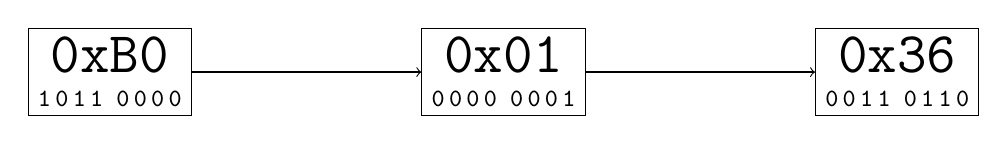
\begin{tikzpicture}
    \texttt{
        \draw (0,0) node[draw, align=center](stsb){
            \huge 0xB0 \\
            \small 1\,0\,1\,1 0\,0\,0\,0
        };
        \draw (5,0) node[draw, align=center](dtb1){
            \huge 0x01 \\
            \small 0\,0\,0\,0 0\,0\,0\,1
        };
        \draw (10,0) node[draw, align=center](dtb2){
            \huge 0x36 \\
            \small 0\,0\,1\,1 0\,1\,1\,0
        };
        \draw[->] (stsb.east) -- (dtb1.west);
        \draw[->] (dtb1.east) -- (dtb2.west);
    }
    \end{tikzpicture}
    \caption{Struktura zprávy \emph{Změna kontroléru} \cite{MIDIspecs}.}
    \label{fig:MIDImsg}
\end{figure}

Z prvního bajtu zprávy z obr. \ref{fig:MIDImsg} lze dekódovat druh a cílový kanál příkazu. Jedná se o \emph{Control Change - Změna kontroléru} na \emph{kanálu 1}\footnote{$0000_2 \sim \mathrm{kanál\ 1}\,\ldots\,1111_2\sim\mathrm{kanál\ 16}$.} Druhý bajt představuje číslo kontroléru (2 -- \emph{Modulation}) a třetí jeho hodnotu (54).

Pro potřeby tohoto semestrálního projektu bude nutné, aby každý přípravek dokázal rozeznat kanál k němu příchozí \acs{MIDI} zprávy, popř. jej pro další přenos pozměnil. \texttt{DATA~BAJTY} budou jen \uv{kopírovány} a nebude se do nich nijak zasahováno.

\subsection{Výjimky}\label{chpt:MIDIexcs}
Je třeba alespoň okrajově zmínit výjimečné stavy, které v rámci \acs{MIDI} protokolu mohou nastat. V této fázi semestrální práce tyto výjimky zatím nejsou ošetřeny.

\subsubsection{Running Status}
Pracuje-li \acs{MIDI} vysílač v tomto stavu, neposílá \texttt{STATUS BAJT} v~opakující se zprávě stejného druhu. Přijímač si tedy musí uložit poslední platný \texttt{STATUS BAJT} do paměti, kterou přemaže, obdrží-li zprávu s jiným, novým \texttt{STATUS BAJTEM}. Tento mód výrazně šetří přenesená data, zejména je-li použit při odesílání zprávy \emph{Změna kontroléru} kontinuálních ovladačů. \cite{MIDIspecs}

\subsubsection{Zprávy Real-Time}
Tyto zprávy slouží pro synchronizaci \acs{MIDI} zařízení, které pracují s časovou osou nebo časem obecně. Skládají se pouze z jediného bajtu a mají nejvyšší prioritu. Přijímač by měl být připraven i na to, že je obdrží uprostřed standardní zprávy nebo SysEx zprávy. \cite{MIDIspecs}

\subsubsection{Zprávy SysEx}
SysEx (\emph{System Exlusive}) zprávy se skládají z většího a libovolného počtu bajtů. Jsou víceúčelové a univerzální, používají se například pro posun na časové ose (komplementárně ke zprávám \textbf{Real-Time}), \acs{MSC}\footnote{\acl{MSC}} apod. \cite{MIDIspecs}

%\section{Softwarová vrstva}
%\begin{circuitikz}
    \draw (0,0) circle(0.5cm) ++ (0,-0.9) node {MIDI OUT};
    \draw (0,0.3) circle(0.07cm) node(midi2){} ++(0.1,0.35) node {\tiny 2};
    \draw (-0.3,0) circle(0.07cm) node(midi3){} ++(-0.35,0) node {\tiny 3};
    \draw (0.3,0) circle(0.07cm) node(midi1){} ++(0.35,0) node {\tiny 1};
    \draw (0.22,0.22) circle(0.07cm) node(midi4){} ++(0.32,0.15) node {\tiny 4};
    \draw (-0.22, 0.22) circle(0.07cm) node(midi5){} ++(-0.32,0.15) node {\tiny 5};
    
    \draw (midi2) -- (0,1.5) to[short,-*] (-1,1.5);
    \draw (midi4) -- (0.7,0.7) -- (0.7,2) -- (-2,2);
    \draw (-4,2) node[left]{\small 5\,V} to[short, o-] ++(0,0) to[R=\footnotesize $220\,\Omega$] (-2,2);
    \draw (midi5) -- (-0.7,0.7) -- (-0.7,1) -- (-2,1);
    \draw (-4,1) to[R=\footnotesize $220\,\Omega$] (-2,1);
    
    \draw[densely dashed] (-1.3,1.5) ellipse (0.3 and 0.9);
    \draw (-1.3,0.6) to[short, -*] ++(0,0) node[ground]{};
    
    \draw (-7,1) to[short,o-] (-6.5,1) to[amp] (-5,1) to[amp, t=\small A] (-4,1);
    \draw (-7,1) node[left]{FROM UART};
    
    
\end{circuitikz}